\documentclass[17pt]{beamer}

\usepackage{amsmath}
\usepackage{mathtools}
\usepackage{listings}
\usepackage{graphicx}

\lstset{
  basicstyle=\scriptsize\ttfamily,
  showstringspaces=false
}

\begin{document}

\title{How To Build Tile Server Using OpenStreetMap tools and data}
\author{Andrii Mishkovskyi}
\date{March 2011}

\maketitle

% \AtBeginSection[] % Do nothing for \section*
% {
%   \begin{frame}<beamer>
%     \frametitle{Outline}
%     \tableofcontents[currentsection]
%   \end{frame}
% }

\AtBeginSubsection[] % Do nothing for \subsection*
{
  \begin{frame}<beamer>
    \frametitle{Outline}
    \scriptsize{\tableofcontents[currentsubsection]}
  \end{frame}
}

\section*{Outline}

\begin{frame}
  \frametitle{Outline}
  \scriptsize{\tableofcontents}
\end{frame}

\section{Objectives and prerequisites}

\begin{frame}{What will you learn?}
  \begin{itemize}
  \item Cartography basics
  \item How to render maps with Mapnik
  \item How to build basic map service with Flask
  \end{itemize}
\end{frame}

\begin{frame}{First of all}
  \begin{itemize}
  \item Grab the CD or flash with all the data from me
  \item Use materials at mishkovskyi.net/pycon2011
  \item Or use handouts
  \end{itemize}
\end{frame}

\section{Introduction}

\subsection{Definitions}

\begin{frame}
  \frametitle{Terms}
  \begin{description}
  \item[Map] \only<1>{Graphic representation of the geographical setting}
  \item[Cartography] \only<2>{Science and practice of making maps}
  \item[Spatial data] \only<3>{Any kind of data linked to location}
  \item[GIS] \only<4>{A system that collects, analyzes, manages or processes in any other way spatial data.}
  \end{description}
\end{frame}

\begin{frame}
  \frametitle{Applications of GIS}
  \begin{itemize}
  \item Geography
  \item Cartography
  \item Navigation
  \item Search engines
  \item Remote sensing, land surveying, urban planning \ldots{}
  \end{itemize}
\end{frame}

\begin{frame}
  \frametitle{Characteristics of maps}
  \begin{itemize}
  \item<1-> Reduction \uncover<2->{\(\implies\) Scale}
  \item<3-> Transformation \uncover<4->{\(\implies\) Map projection}
  \item<5-> Abstractions \uncover<6->{\(\implies\) Symbolism}
  \end{itemize}
\end{frame}

% TODO: elaborate, more keywords
\begin{frame}
  \frametitle{Classification of maps}
  \begin{description}
  \item[Scale] \only<1>{Relative size at which objects are represented
      \begin{itemize}
      \item Small-scale -- map of the world or continent
      \item Large-scale -- map of your neighborhood
      \end{itemize}
    }
  \item[Function] \only<2>{
      \begin{itemize}
      \item General reference
      \item Thematic
      \item Charts
      \end{itemize}
    }
  \item[Subject matter] \only<3>{
      \begin{itemize}
      \item Cadastre
      \item Plans
      \end{itemize}
    }
  \end{description}
\end{frame}


\subsection{Map projections}

% TODO: Add image
\begin{frame}
  \frametitle{Projection}
  Conversion of spherical information into two dimensional pane.
\end{frame}

% TODO: add images

\begin{frame}
  \frametitle{Patterns of distortion}
  \begin{itemize}
  \item Azimuthal
  \item Conical
  \item Cylindrical
  \end{itemize}
\end{frame}

\begin{frame}
  \frametitle{Characteristics of projection}
  \begin{itemize}
  \item Angle distortion
  \item Area distortion
  \item Linear distortion (scale factor)
  \item Direction distortion
  \end{itemize}
\end{frame}

\begin{frame}
  \frametitle{Tissot indicatrix}
  \begin{block}{Representation of map distortions}
    \begin{center}
      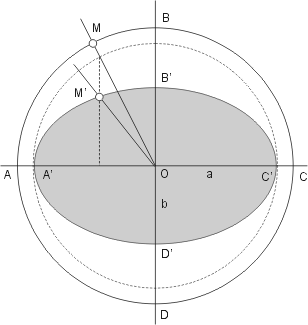
\includegraphics[scale=0.5]{pycon-2011-tutorial-files/indicatrix.png}
    \end{center}
  \end{block}
\end{frame}

\begin{frame}
  \frametitle{Mercator projection}
\only<2>{
  \begin{center}
    \begin{block}{Description}
      \begin{itemize}
      \item Conformal cylindrical projection
      \item No angle distortion
      \item Major area and linear distortion around poles
      \item Historically used for navigation
      \end{itemize}
    \end{block}
  \end{center}
}
\only<1>{
  \begin{block}{Tissot's indicatrix}
    \begin{center}
      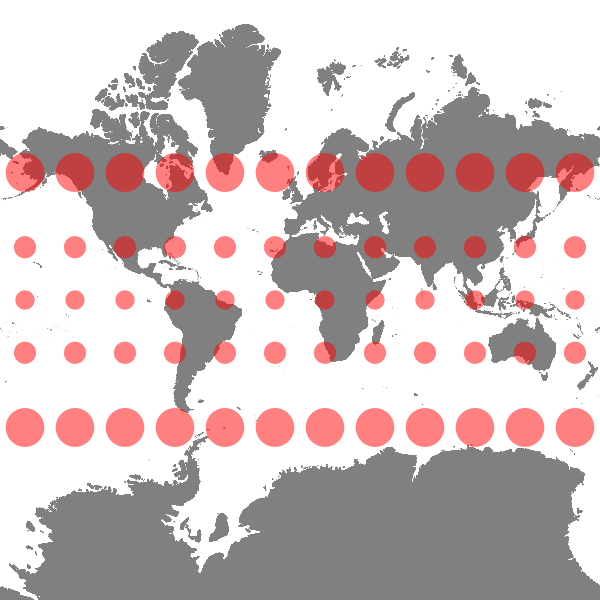
\includegraphics[scale=0.25]{pycon-2011-tutorial-files/merc-indicatrix.png}
    \end{center}
  \end{block}
}
\end{frame}

\begin{frame}
  \frametitle{Mollweide Projection}
\only<2>{
  \begin{block}{Description}
    \begin{itemize}
    \item Pseudocylindrical equal-area projection
    \item Serious linear and angle distortion
    \item Useful where area size is important (global distributions, visual
      area size comparison, etc)
    \end{itemize}
  \end{block}
}
\only<1>{
  \begin{block}{Tissot's indicatrix}
    \begin{center}
      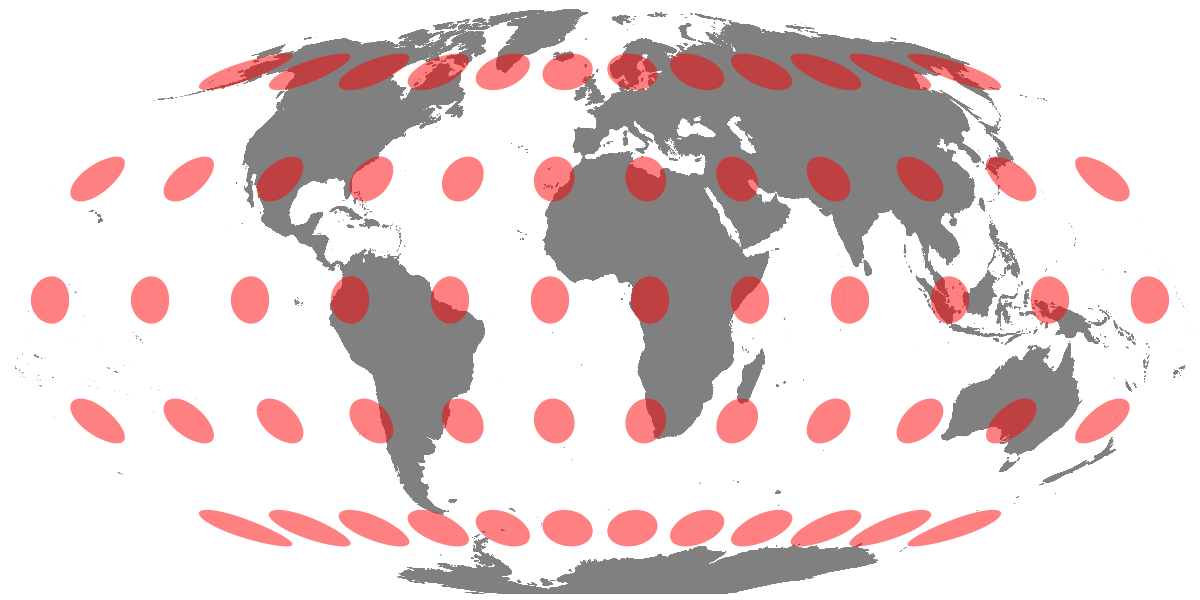
\includegraphics[scale=0.25]{pycon-2011-tutorial-files/moll-indicatrix.png}
    \end{center}
  \end{block}
}
\end{frame}

\subsection{Spatial data}

% TODO: expand

\begin{frame}
  \frametitle{Classes of data}
  \begin{itemize}
  \item Physical (Topographical -- elevations, terrain \& water objects)
  \item Cultural
  \item Human-made
  \end{itemize}
\end{frame}

\begin{frame}
  \frametitle{Sources of data}
  \begin{itemize}
  \item Mapping companies (TeleAtlas, Navteq, Ordnance Survey)
  \item Public sources (OpenStreetMap, Natural Earth)
  \item Government institutions (NASA, local government)
  \item Personal data (GPS tracks, social networks)
  \end{itemize}
\end{frame}

\begin{frame}
  \frametitle{Collecting data}
  \begin{itemize}
  \item Surveying
  \item GPS tracks
  \item Aerial imagery
  \end{itemize}
\end{frame}

\begin{frame}
  \frametitle{Storing data}
  \begin{itemize}
  \item RDBMS (PostgreSQL + PostGIS, MySQL Spatial, Oracle Spatial, Spatialite)
  \item Non-relational databases (Neo4j, MongoDB, CouchDB)
  \item Flat files (Shapefiles, GeoJSON, KML, GML)
  \end{itemize}
\end{frame}

\begin{frame}
  \frametitle{Simple Feature acess: SQL}
  \begin{itemize}
  \item Full set of querying functions
  \item Tons of useful features for on-the-fly projecting etc.
  \item Almost fully supported by PostGIS
  \end{itemize}
\end{frame}

\begin{frame}
  \frametitle{Other standards}
  \begin{itemize}
  \item Well-known text/binary
  \item Keyhole Markup Language
  \item Geography Markup Language
  \item Esri Shapefiles
  \end{itemize}
\end{frame}

\begin{frame}
  \frametitle{How OSM handles data}
  Special XML format used in
  \begin{itemize}
  \item Official API
  \item Official planet extracts
  \item Unofficial eXtended API (XAPI)
  \end{itemize}
\end{frame}

\begin{frame}[t]
  \frametitle{OSM data primitives}
  \begin{description}
  \item[Node] \only<1>{Stands for one geospatial point.}
  \item[Way] \only<2>{Collection of nodes. Can be used to represent
    such geometric features as lines (roads, borders, etc)
    and polygons (parks, buildings, etc.).}
  \item[Relation] \only<3>{Collection of other primitives (including
    relations themselves). Used for storing complex
    relationships between geospatial objects.}
  \end{description}
\end{frame}

\begin{frame}[fragile]
  \frametitle{How OSM XML looks like}
  \lstinputlisting[language=XML]{osm-xml-overview.xml}
\end{frame}

\begin{frame}
  \frametitle{Nodes}
  \lstinputlisting[language=XML]{osm-nodes-overview.xml}
\end{frame}

\begin{frame}
  \frametitle{Ways}
  \lstinputlisting[language=XML]{osm-ways-overview.xml}
\end{frame}

% TODO: Add nodes?

\begin{frame}
  \frametitle{Relations}
  \lstinputlisting[language=XML]{osm-relations-overview.xml}
\end{frame}

\begin{frame}
  \frametitle{Parsing OSM data}
  \begin{itemize}
  \item osm2pgsql
  \item Osmosis
  \item imposm
  \item osm2ogr, osm2shp, \ldots
  \end{itemize}
\end{frame}

% TODO: FINISH

\begin{frame}
  \frametitle{Importing data using osm2pgsql}
  \texttt{\$ osm2pgsql -S import.style -d gis -m georgia.osm.bz2}
  \begin{description}
  \item[-S] \only<1>{Path to style file for osm2pgsql, which defines how and what data will be imported}
  \item[-d] \only<2>{Database name}
  \item[-m] \only<3>{Import data in Mercator projection}
  \end{description}
\end{frame}

\begin{frame}[t]
  \frametitle{Table layout after osm2pgsql import}
  \begin{description}
  \item[planet\_osm\_point] \only<2>{Stores features which are represented with single symbol,
    such as bus stops, hotels (if mapped as points), ATMs, etc.}
  \item[planet\_osm\_line] \only<3>{Almost 90\% is take by different types of roads.}
  \item[planet\_osm\_polygon] \only<4>{Buildings, parks, etc.}
  \end{description}
\end{frame}

\section{Mapnik}

\subsection*{Introduction}

\begin{frame}
  \frametitle{What is Mapnik}
  Map rendering framework, written in \texttt{C++} with built-in \texttt{Python} bindings.
\end{frame}

\begin{frame}
  \frametitle{Mapnik concepts}
  \begin{description}
  \item[Symbolizer] \only<1>{Drawing rule of given geometric feature}
  \item[Rule] \only<2>{Collection of symbolizers for various data inputs.}
  \item[Style] \only<3>{Collection of rules. Exists mostly of convenience
    for defining layers.}
  \item[Datasource] \only<4>{Source of geospatial data.}
  \item[Layer] \only<5>{Description of which style will be used to render
    given datasource}
  \item[Map] \only<6>{Container of layers and styles}
  \end{description}
\end{frame}

% TODO: add picture of map + layer + styles

\subsection{Hello World in Mapnik}

\begin{frame}
  \frametitle{Rendering map}
  \only<1>{
    \begin{center}
      \lstinputlisting{pycon-2011-tutorial-files/hw-import.py}
    \end{center}
  }
  \only<2>{
    \begin{center}
      \lstinputlisting{pycon-2011-tutorial-files/hw-rules.py}
    \end{center}
  }
  \only<3>{
    \begin{center}
      \lstinputlisting{pycon-2011-tutorial-files/hw-styles.py}
    \end{center}
  }
  \only<4>{
    \begin{center}
      \lstinputlisting{pycon-2011-tutorial-files/hw-layers.py}
    \end{center}
  }
  \only<5>{
    \begin{center}
      \lstinputlisting{pycon-2011-tutorial-files/hw-map.py}
    \end{center}
  }
  \only<6>{
    \begin{center}
      \lstinputlisting{pycon-2011-tutorial-files/hw-image.py}
    \end{center}
  }
  \only<7>{
    \begin{block}{Result}
      \begin{center}
        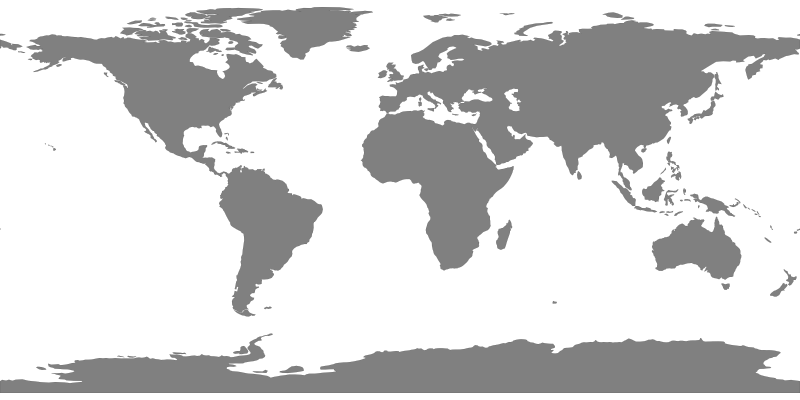
\includegraphics[scale=0.4]{pycon-2011-tutorial-files/hw.png}
      \end{center}
    \end{block}
  }
\end{frame}

% TODO: finish

\begin{frame}
  \frametitle{Map and Image size}
  \begin{itemize}
  \item As you might remember, we've set width and
    height to both Map and Image
  \item The concept of map view and bounding box
  \end{itemize}
\end{frame}

\subsection{Handling projections in Mapnik}

% TODO: finish

\begin{frame}
  \frametitle{Projections in Mapnik}
  \only<1>{
    \begin{itemize}
    \item Provided by Proj.4 library
      TODO: add explanation, provide examples
    \end{itemize}
  }
  \only<2>{
    To make sure you don't make any mistakes,
    use \texttt{spatialreference.org}.
  }
\end{frame}

\subsection{Using XML in Mapnik}

\begin{frame}
  \frametitle{Creating map file}
  \only<1>{
    \begin{center}
      \lstinputlisting{pycon-2011-tutorial-files/hw-map.xml}
    \end{center}
  }
  \only<2>{
    \begin{center}
      \lstinputlisting{pycon-2011-tutorial-files/hw-style.xml}
    \end{center}
  }
  \only<3>{
    \begin{center}
      \lstinputlisting{pycon-2011-tutorial-files/hw-layer.xml}
    \end{center}
  }
\end{frame}

\begin{frame}
  \frametitle{Loading map file}
  \only<1>{
    \begin{block}{Imports}
      \begin{center}
        \lstinputlisting{pycon-2011-tutorial-files/hw-xml-import.py}
      \end{center}
    \end{block}
  }
  \only<2>{
    \begin{block}{Rendering}
      \begin{center}
        \lstinputlisting{pycon-2011-tutorial-files/hw-image-crippled.py}
      \end{center}
    \end{block}
  }
  \only<3>{
    \begin{block}{Result}
      \begin{center}
        
\includegraphics[scale=0.3]{pycon-2011-tutorial-files/hw-crippled.png}
      \end{center}
    \end{block}
  }
  \only<4>{
    \begin{block}{What's wrong?}
      \begin{center}
        \lstinputlisting{pycon-2011-tutorial-files/hw-where-wrong.py}
      \end{center}
    \end{block}
  }
\end{frame}

\begin{frame}
  \frametitle{Fixing the image}
  \only<1>{
    \begin{block}{Importing}
      \begin{center}
        \lstinputlisting{pycon-2011-tutorial-files/hw-xml-import-fixed.py}
      \end{center}
    \end{block}
  }
  \only<2>{
    \begin{block}{Creating projection}
      \begin{center}
        \lstinputlisting{pycon-2011-tutorial-files/hw-proj.py}
      \end{center}
    \end{block}
  }
  \only<3>{
    \begin{block}{Setting bounding box}
      \begin{center}
        \lstinputlisting{pycon-2011-tutorial-files/hw-bbox.py}
      \end{center}
    \end{block}
  }
  \only<4>{
    \begin{block}{Rendering}
      \begin{center}
        \lstinputlisting{pycon-2011-tutorial-files/hw-image-fixed.py}
      \end{center}
    \end{block}
  }
  \only<5>{
    \begin{block}{Result}
      \begin{center}
        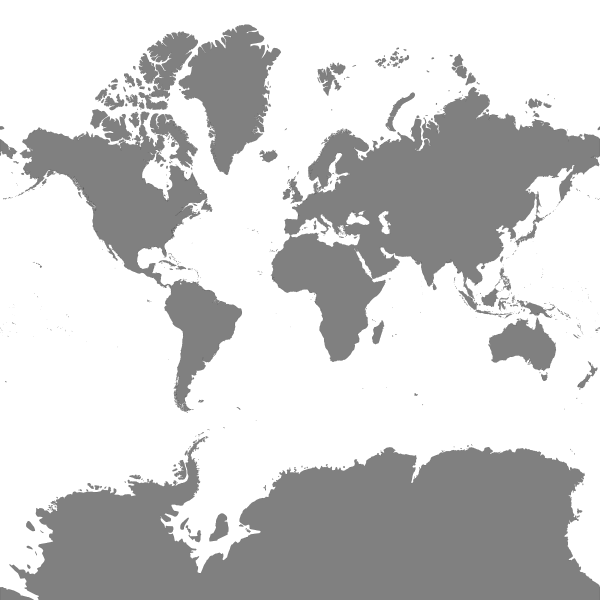
\includegraphics[scale=0.3]{pycon-2011-tutorial-files/hw-fixed.png}
      \end{center}
    \end{block}
  }
\end{frame}

\subsection{More on Mapnik XML}

\begin{frame}
  \frametitle{SQL mini-tutorial}
  \lstinputlisting{pycon-2011-tutorial-files/find-hyatt.sql}

  \lstinputlisting{pycon-2011-tutorial-files/find-hyatt-with-bbox.sql}
  \lstinputlisting{pycon-2011-tutorial-files/find-hyatt-with-bbox-and-reprojection.sql}
\end{frame}

\begin{frame}
  \frametitle{Extending map files}
  \only<1>{
    \begin{block}{Changing rules based on scale}
      \begin{center}
        \lstinputlisting[language=XML]{pycon-2011-tutorial-files/ext-scale.xml}
      \end{center}
    \end{block}
  }
  \only<2>{
    \begin{block}{Changing rules based on tags}
      \begin{center}
        \lstinputlisting[language=XML]{pycon-2011-tutorial-files/ext-filter.xml}
      \end{center}
    \end{block}
  }
  \only<3>{
    \begin{block}{Adding point symbols}
      \begin{center}
        \lstinputlisting[language=XML]{pycon-2011-tutorial-files/ext-point.xml}
      \end{center}
    \end{block}
  }
  \only<4>{
    \begin{block}{Adding PostGIS datasource}
      \begin{center}
        \lstinputlisting[language=XML]{pycon-2011-tutorial-files/ext-postgis.xml}
      \end{center}
    \end{block}
  }
  \only<5>{
    \begin{block}{Drawing ATMs}
      \begin{center}
        \lstinputlisting[language=XML]{pycon-2011-tutorial-files/ext-atm.xml}
      \end{center}
    \end{block}
  }
  \only<6>{
    \begin{block}{Drawing ATMs}
      \begin{center}
        \lstinputlisting[language=XML]{pycon-2011-tutorial-files/ext-atm-layer.xml}
      \end{center}
    \end{block}
  }
  \only<7>{
    \begin{center}{Adding hotels}
      \lstinputlisting[language=XML]{pycon-2011-tutorial-files/ext-hotels.xml}
    \end{center}
  }
  % \only<>{
  %   \begin{center}
  %     \lstinputlisting[language=XML]{pycon-2011-tutorial-files/ext-roads.xml}
  %   \end{center}
  % }
  % \only<>{
  %   \begin{center}
  %     \lstinputlisting[language=XML]{pycon-2011-tutorial-files/ext-extent.xml}
  %   \end{center}
  % }
  % \only<>{
  %   \begin{center}
  %     \lstinputlisting[language=XML]{pycon-2011-tutorial-files/ext-postgis.xml}
  %   \end{center}
  % }
  % \only<>{
  %   \begin{center}
  %     \lstinputlisting[language=XML]{pycon-2011-tutorial-files/ext-text.xml}
  %   \end{center}
  % }
  % \only<>{
  %   \begin{center}
  %     \lstinputlisting[language=XML]{pycon-2011-tutorial-files/ext-parking.xml}
  %   \end{center}
  % }
  % \only<>{
  %   \begin{center}
  %     \lstinputlisting[language=XML]{pycon-2011-tutorial-files/ext-hotels.xml}
  %   \end{center}
  % }
  % \only<>{
  %   \begin{center}
  %     \lstinputlisting[language=XML]{pycon-2011-tutorial-files/ext-buildings.xml}
  %   \end{center}
  % }
  % \only<>{
  %   \begin{center}
  %     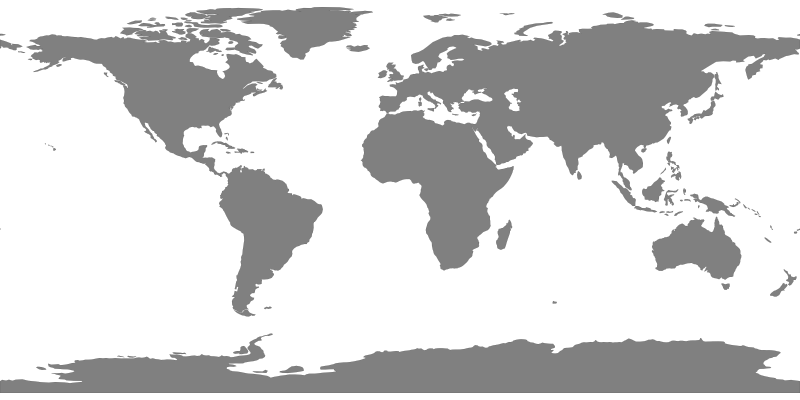
\includegraphics{pycon-2011-tutorial-files/extended.png}
  %   \end{center}
  % }
\end{frame}


% \subsection{Mapnik map files}

% \begin{frame}
%   \frametitle{Overview of map file in XML}

% \end{frame}

% \begin{frame}
%   \frametitle{Defining styles in XML}

% \end{frame}

% \begin{frame}
%   \frametitle{Defining rules in XML}

% \end{frame}

% \begin{frame}
%   \frametitle{Defining layers in XML}

% \end{frame}

% \subsection{Real world example}

% \begin{frame}
%   \frametitle{Fonts and fontsets}

% \end{frame}

% \begin{frame}
%   \frametitle{Including PostGIS datasources}

% \end{frame}

% \begin{frame}
%   \frametitle{Changing level of details aka zoom levels}

% \end{frame}

% \begin{frame}
%   \frametitle{Adding roads}

% \end{frame}


% \begin{frame}
%   \frametitle{Adding POIs}

% \end{frame}


\section{Imagery server}

\begin{frame}
  \frametitle{Our goals}

\end{frame}

\subsection{Simple map requests}

\begin{frame}[fragile]
  \frametitle{Hello world API}
  \begin{block}{\ttfamily{http://localhost:5000/map}}
    \only<1>{
      \lstinputlisting{pycon-2011-tutorial-files/ts-hw-import.py}
    }
    \only<2>{
      \lstinputlisting{pycon-2011-tutorial-files/ts-hw-handler.py}
    }
    \only<3>{
      \lstinputlisting{pycon-2011-tutorial-files/ts-hw-utils-render.py}
    }
  \end{block}
\end{frame}

\subsection{Tile API}

\begin{frame}
  \frametitle{What are tiles}

\end{frame}

\begin{frame}[fragile]
  \frametitle{Tile API}
  \begin{block}{\ttfamily{http://localhost:5000/0/0/0.png}}
    \only<1>{
      \lstinputlisting{pycon-2011-tutorial-files/ts-hw-tile-import.py}
    }
    \only<2>{
      \lstinputlisting{pycon-2011-tutorial-files/ts-hw-tile.py}
    }
    \only<3>{
      \lstinputlisting{pycon-2011-tutorial-files/ts-hw-utils-parse_coords.py}
    }
    \only<4>{
      \lstinputlisting{pycon-2011-tutorial-files/ts-hw-utils-pixel2latlon.py}
    }
  \end{block}
\end{frame}

\subsection{Staticmaps API}

\subsection{Utility APIs}

\begin{frame}
  \frametitle{pixel2latlon}

\end{frame}

\begin{frame}
  \frametitle{latlon2pixel}

\end{frame}

\begin{frame}
  \frametitle{latlon2tile \& tile2latlon}

\end{frame}

\begin{frame}
  \frametitle{tilesbbox}

\end{frame}

\section*{Summary}

\begin{frame}
  \frametitle{What's been left behind?}
  \begin{itemize}
  \item Usage of PolygonPatternSymbolizer and LinePatternSymbolizer
  \item Handling of huge XML files through entities
  \item Database optimizations
  \end{itemize}
\end{frame}

\begin{frame}
  \frametitle{What to do next?}
  \begin{itemize}
  \item Build your own specialized map
  \item Experiment with Mapnik 2.0
  \item Get into Mapnik development
  \end{itemize}
\end{frame}

\begin{frame}
  \frametitle{Wrapping up}
  \begin{itemize}
  \item Hope you have learned something useful and new
  \item Contact me at \texttt{contact@mishkovskyi.net}
  \end{itemize}
\end{frame}

% http://msdn.microsoft.com/en-us/library/bb259689.aspx

\end{document}
